\section{Preliminary studies}

This section carries out some preliminary studies using Moltres and MOOSE heat conduction module to solve the prismatic HTGR thermal-fluids.

\subsection{Verification of the thermal-fluids model}

To verify our methodology, this section solved a simplified cylindrical model whose analytical solution we know.
Section \ref{appendix:ver} presents the analytical solution of the problem.
Moltres/MOOSE obtained the numerical solution of the thermal-fluid equations from Section \ref{ch3:th}.

Figure \ref{fig:th-ver-mesh} displays the model geometry, which differentiates five subregions: fuel compact, helium gap, moderator, film, and coolant.
Table \ref{tab:th-ver-char} summarizes the geometry dimensions and the input parameters.
The model reference design was the GT-MHR.
The calculated moderator radius is the fuel/coolant pitch minus the fuel compact and coolant channel radii, which is the minimum distance between the fuel and coolant channels in the unit cell.
We obtained the calculated coolant radius by preserves the coolant channel volume.
The model assumed a sinusoidal power profile in the $z$-direction.

\begin{figure}[htbp!]
	\centering
	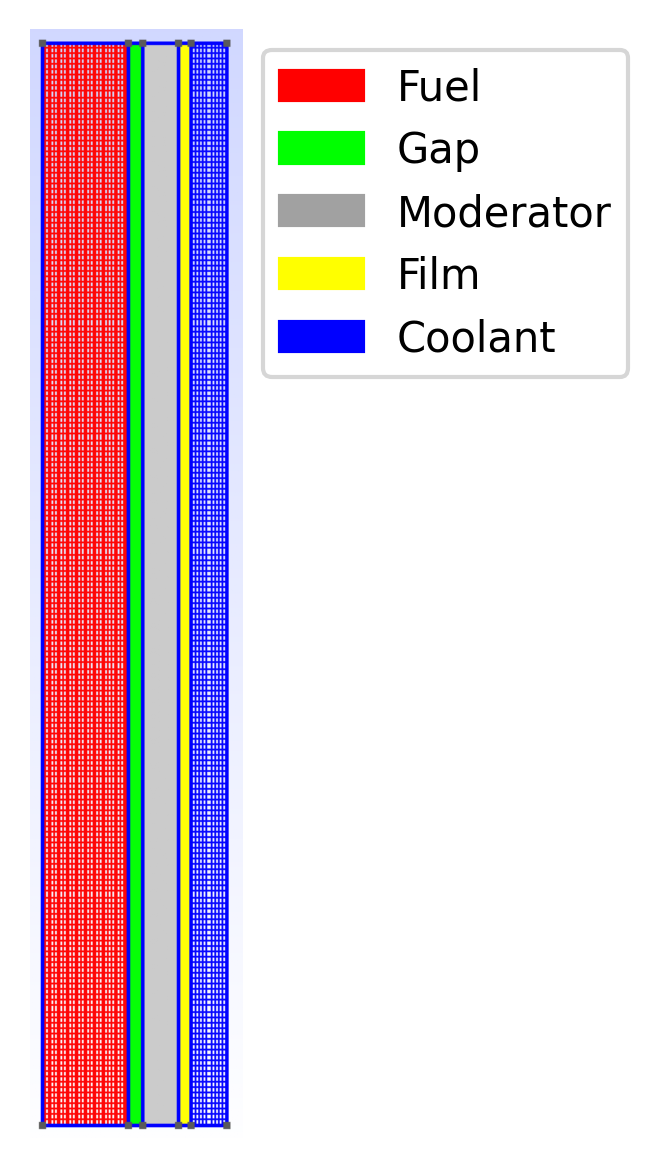
\includegraphics[width=0.25\linewidth]{figures-thermal/2D-preliminar-mesh2}
	\hfill
	\caption{Scaled-down version of the model geometry.}
	\label{fig:th-ver-mesh}
\end{figure}

\begin{table}[htbp!]
\centering
      \caption{Problem characteristics.}
      \label{tab:th-ver-char}
    % \begin{tabular}{@{}l c S[table-format=2.2] c c}
    \begin{tabular}{@{}l c c c c}
    \toprule
    \multicolumn{1}{c}{Parameter} & \multicolumn{1}{c}{Symbol} & \multicolumn{1}{c@{}}{Value} & \multicolumn{1}{c@{}}{Units} & \multicolumn{1}{c}{Reference} \\
    \midrule
  Fuel compact radius   & R$_f$     & 0.6225  & cm       & \cite{in_three-dimensional_2006} \\
  Fuel channel radius   & R$_g$     & 0.6350  & cm       & \cite{in_three-dimensional_2006} \\
  Coolant channel radius   & - 		& 0.7950  & cm       & \cite{in_three-dimensional_2006} \\
  Fuel/coolant pitch    & -			& 1.8850  & cm       & \cite{in_three-dimensional_2006} \\
  Fuel column height	& L 		& 793 	  & cm 		 & \cite{in_three-dimensional_2006} \\
  Coolant mass flow rate & $\dot{m}$ & 0.0176 & kg/s 	 & \cite{in_three-dimensional_2006} \\
  Average power density & q$_{ave}$ & 35      & W/cm$^3$ & \cite{in_three-dimensional_2006} \\
  Coolant inlet temperature 	& $T_{in}$ & 400  & $^{\circ}C$ & \cite{in_three-dimensional_2006} \\
  Helium inlet pressure & P 		& 70      & bar 	 & \cite{in_three-dimensional_2006} \\
  Helium density		& $\rho_c$  & 4.940 $\times 10^{-6}$ & kg/cm$^3$ & \cite{nist_thermophysical_2020} \\
  Helium heat capacity  & c$_{p,c}$	& 5188 & J/kg/K  & \cite{nist_thermophysical_2020} \\
  Fuel compact thermal conductivity & k$_f$ & 0.07    & W/cm/K & \cite{tak_numerical_2008} \\
  Gap thermal conductivity & k$_g$ & 3 $\times 10^{-3}$ & W/cm/K & \cite{tak_numerical_2008} \\
  Moderator thermal conductivity & k$_m$ & 0.30 & W/cm/K 	& \cite{tak_numerical_2008} \\
    \midrule
  \multicolumn{1}{c}{Calculated parameters} &  &  &  & \\  
    \midrule
  Calculated moderator radius 	& R$_m$ & 1.080  	& cm     & - \\
  Coolant film radius   		& R$_i$ & 1.090  	& cm     & - \\
  Calculated coolant radius 	& R$_c$ & 1.349  	& cm     & - \\
  Coolant average velocity  	& v$_c$ & 1794.33 	& cm/s   & - \\
  Film thermal conductivity  	& k$_i$ & 1.722 $\times 10^{-3}$ & W/cm/K & - \\
  \bottomrule
  \end{tabular}
\end{table}

Figure \ref{fig:th-ver-results} shows the axial and radial temperature profiles.
Both analytical and numerical solutions exhibit good agreement.
The outlet coolant temperature is 770.2 $^{\circ}$C whereas the average outlet coolant temperature of the VHTR is 950 $^{\circ}$C.
Note that this is a simplified model only for verification purposes, and it considers only one fuel channel while in the GT-MHR unit cell two fuel channels deposit their heat into one coolant channel.

\begin{figure}[htbp!]
	\centering
    \subfloat[Fuel centerline and bulk coolant axial temperatures.]{
        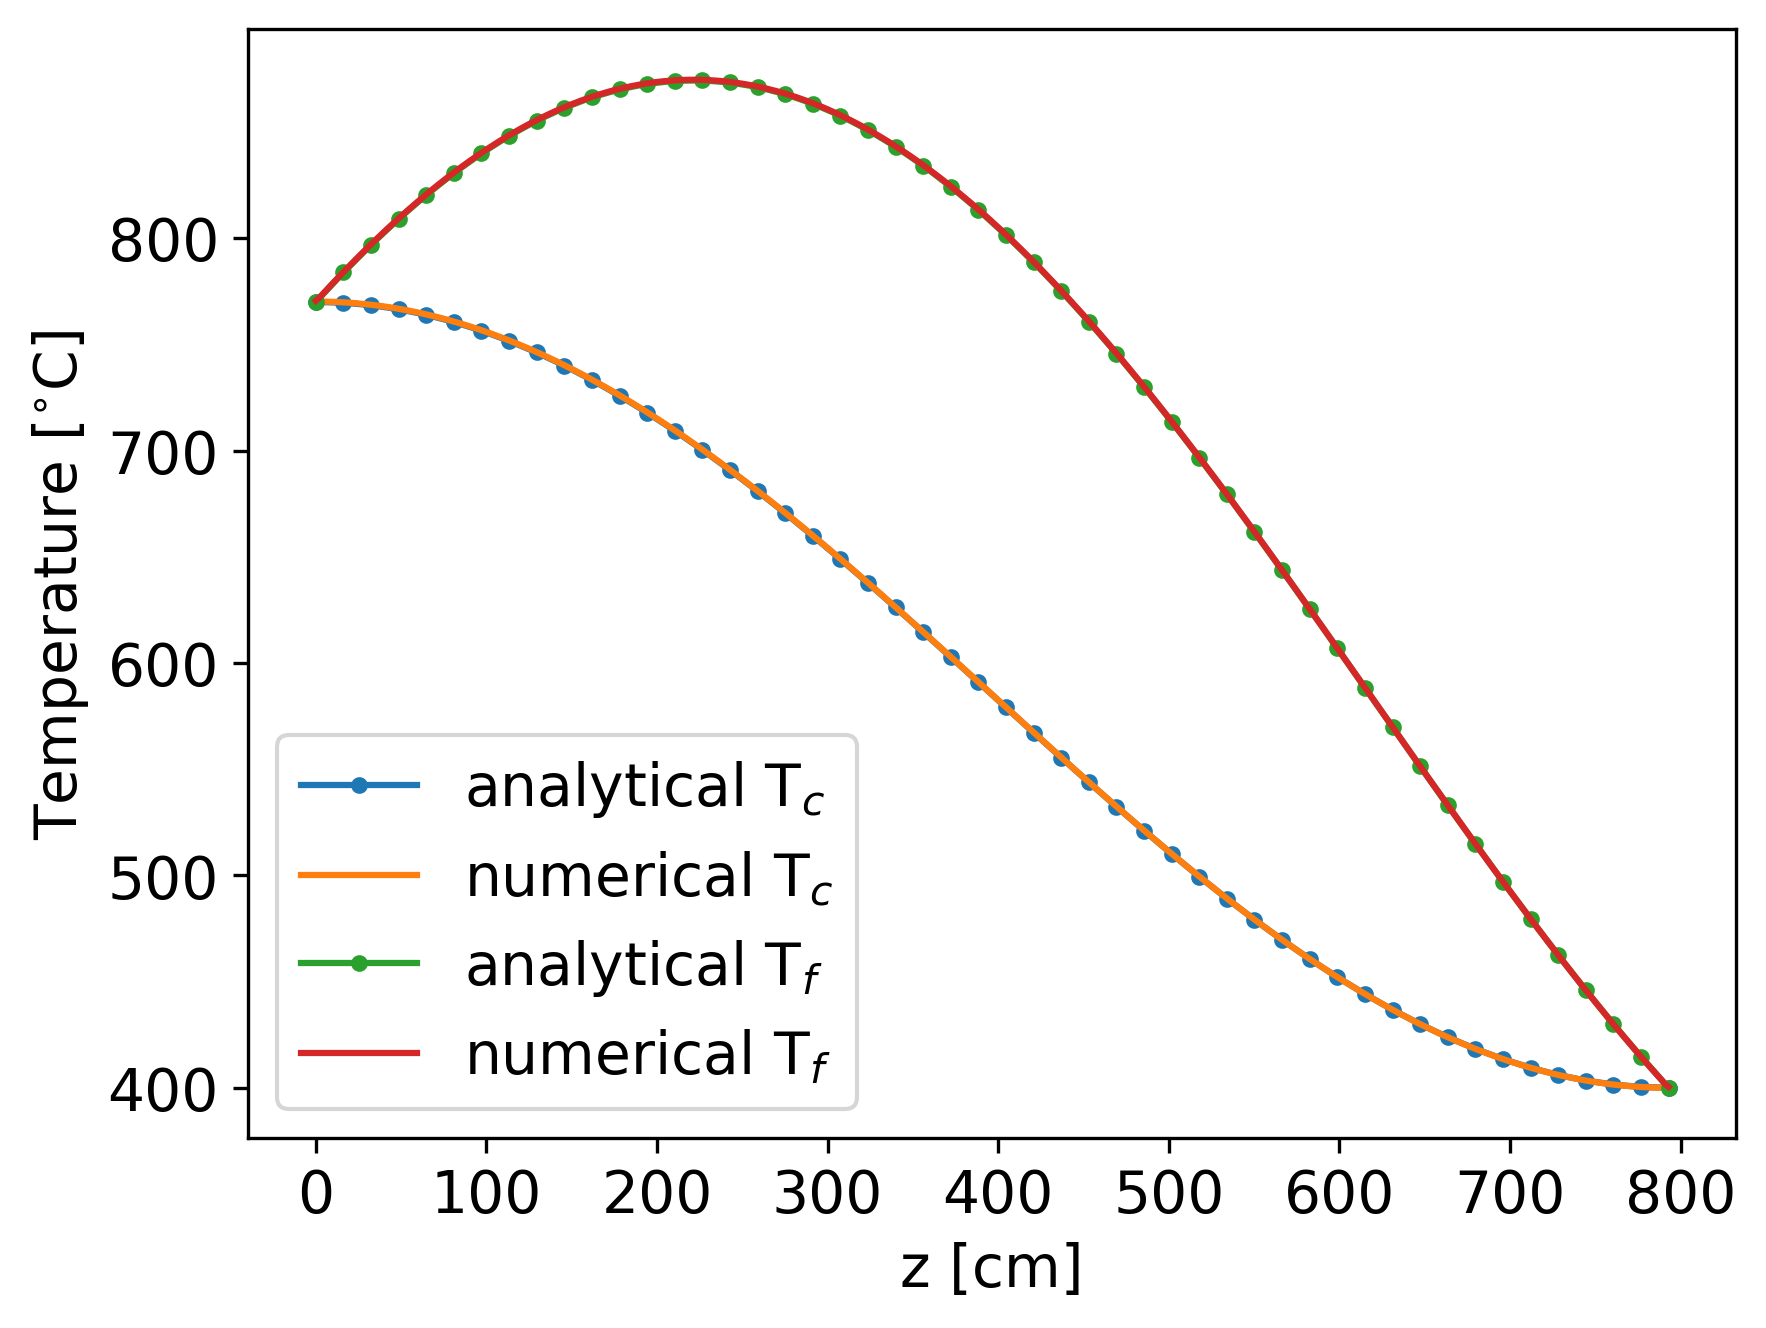
\includegraphics[width=0.45\textwidth]{figures-thermal/2D-preliminar-axial}
    }
    \subfloat[Radial temperature at z=L/2=396.5 cm.]{
        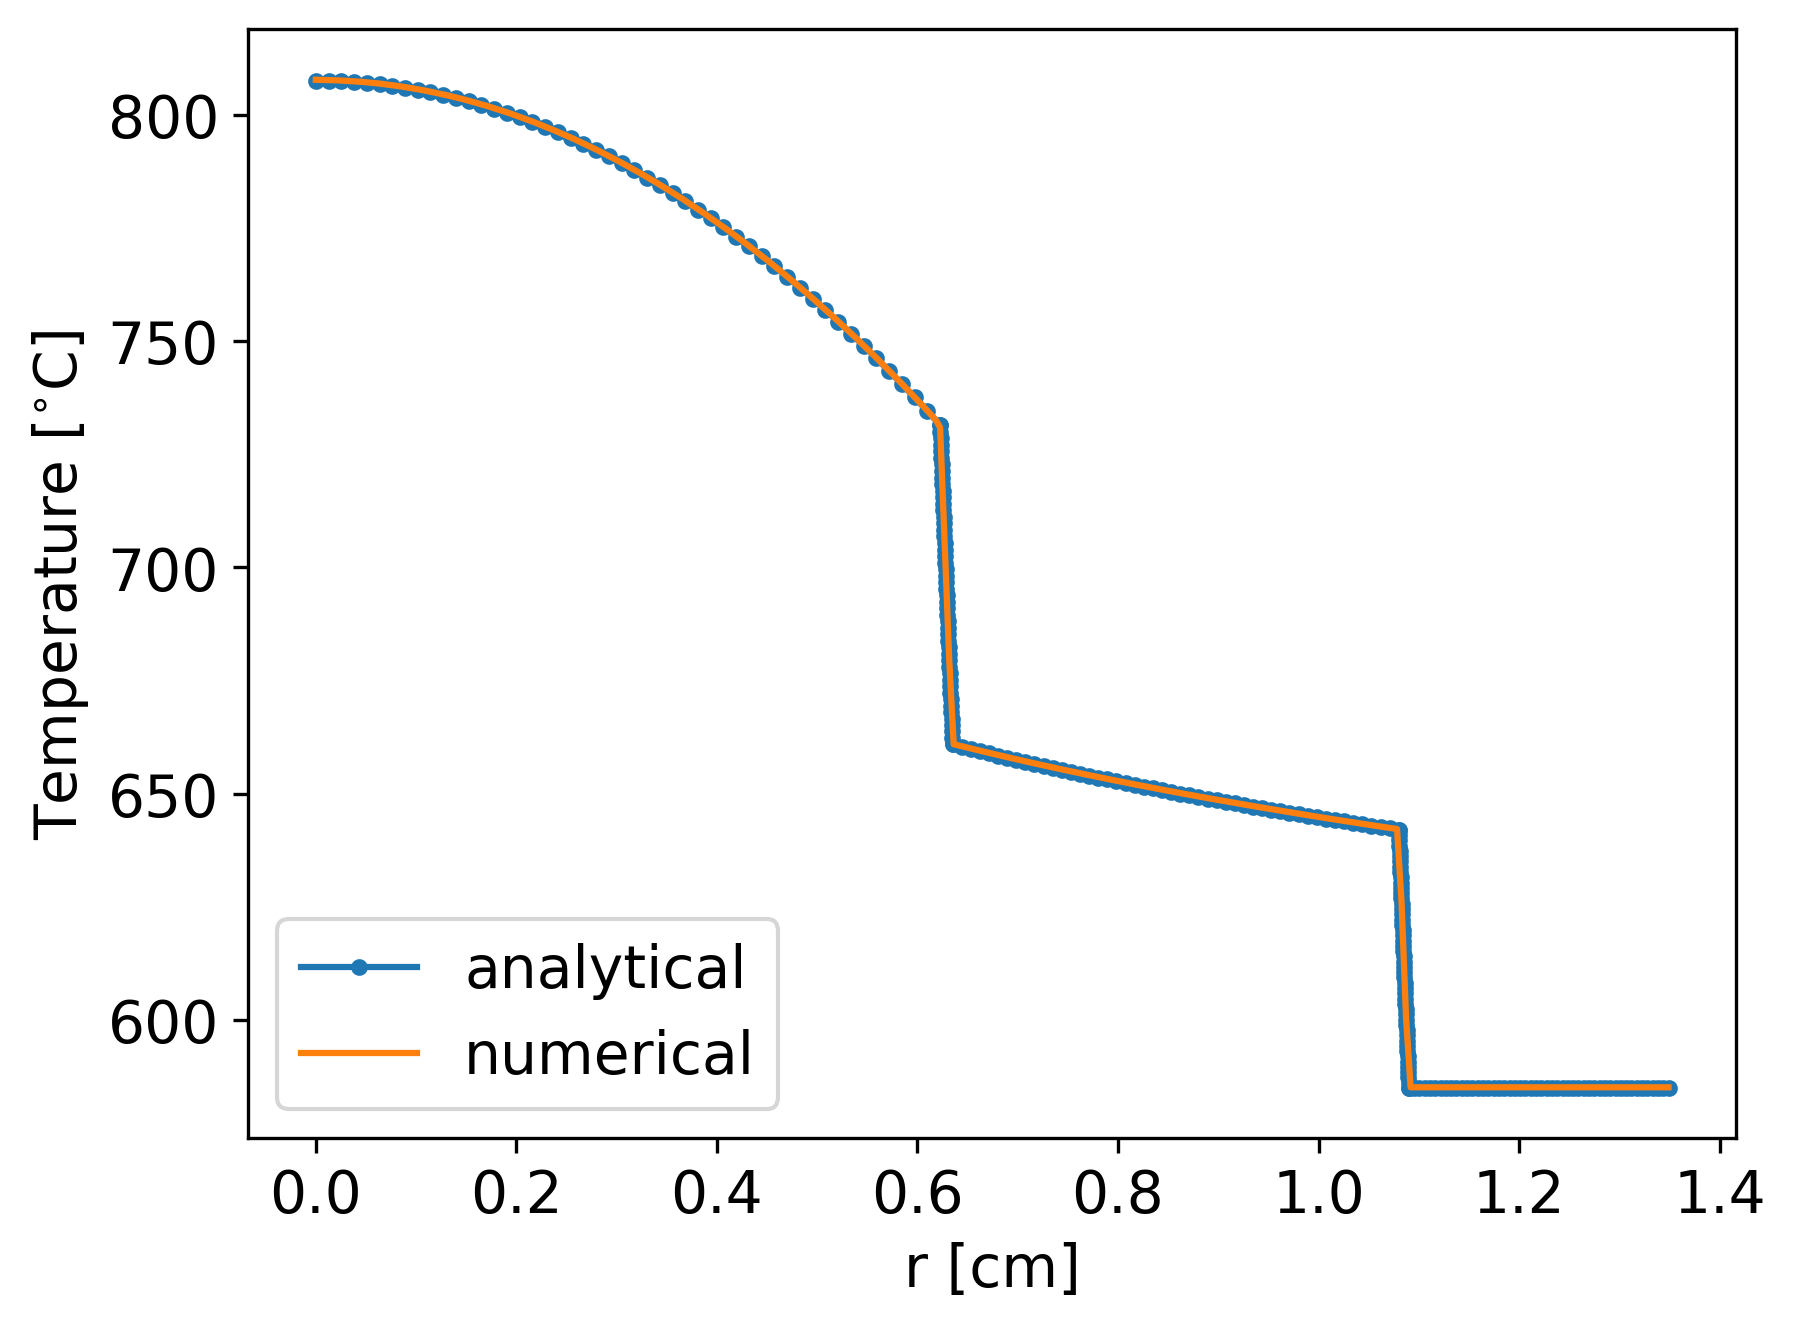
\includegraphics[width=0.45\textwidth]{figures-thermal/2D-preliminar-radial2}
    }
	\hfill
    \caption{Temperature profiles.}
	\label{fig:th-ver-results}
\end{figure}

\section{Unit cell problem}

This section solved the unit cell problem in the hot spot of an HTGR.
We intended to reproduce In et al. 2006 \cite{in_three-dimensional_2006} in an effort for validating the model.
We chose this article as it solves a three-dimensional unit-cell model gives one of the most complete descriptions in the open literature.
Table \ref{tab:th-val-unit-char} presents the problem characteristics.
The material properties specification of the solids is missing in the article, and we replaced them with parameters from Tak et al. 2008 \cite{tak_numerical_2008}.
Figure \ref{fig:th-val-unit-model} displays a $XY$-plane of the model geometry and the material properties that depend on the temperature.
Additionally, In et al. used a chopped cosine as the power profile.
To simplify the analysis, we used the average value of the power profile.

\begin{table}[htbp!]
\centering
      \caption{Problem characteristics.}
      \label{tab:th-val-unit-char}
    % \begin{tabular}{@{}l c S[table-format=2.2] c c}
    \begin{tabular}{@{}l c c c c}
    \toprule
    \multicolumn{1}{c}{Parameter} & \multicolumn{1}{c}{Symbol} & \multicolumn{1}{c@{}}{Value} & \multicolumn{1}{c@{}}{Units} & \multicolumn{1}{c}{Reference} \\
    \midrule
  Fuel compact radius       & R$_f$ & 0.6225    & cm   & \cite{in_three-dimensional_2006} \\
  Fuel channel radius       & R$_g$ & 0.6350    & cm   & \cite{in_three-dimensional_2006} \\
  Coolant channel radius    & R$_c$ & 0.7950    & cm   & \cite{in_three-dimensional_2006} \\
  Fuel/coolant pitch        & p     & 1.8850    & cm   & \cite{in_three-dimensional_2006} \\
  Fuel column height        & L     & 793       & cm   & \cite{in_three-dimensional_2006} \\
  % input parameter characteristics
  Coolant channel mass flow rate & $\dot{m}$ & 0.0176 & kg/s & \cite{in_three-dimensional_2006} \\
  Average power density     & q$_{ave}$ & 35    & W/cm$^3$   & \cite{in_three-dimensional_2006} \\
  Inlet coolant temperature & T$_{in}$  & 400   & $^{\circ}$C  & \cite{in_three-dimensional_2006} \\
  Helium inlet pressure & P & 70 & bar & \cite{in_three-dimensional_2006} \\
  Helium density        & $\rho$  & 4.94 $\times 10^{-6}$ & kg/cm$^3$ & \cite{nist_thermophysical_2020} \\
  Helium heat capacity  & c$_p$ & 5188 & J/kg/K & \cite{nist_thermophysical_2020} \\
    \midrule
  \multicolumn{1}{c}{Calculated parameters} &  &  &  & \\  
    \midrule
  Coolant film radius       & R$_i$ & 0.8050    & cm     & -  \\
  Coolant average velocity  & v$_c$ & 1794.33   & cm/s   & -  \\
  Film thermal conductivity & k$_i$ & 1.731 $\times 10^{-3}$ & W/cm/K & -  \\
  \bottomrule
  \end{tabular}
\end{table}

\begin{figure}[htbp!]
	\centering
    \subfloat[Model geometry.]{
        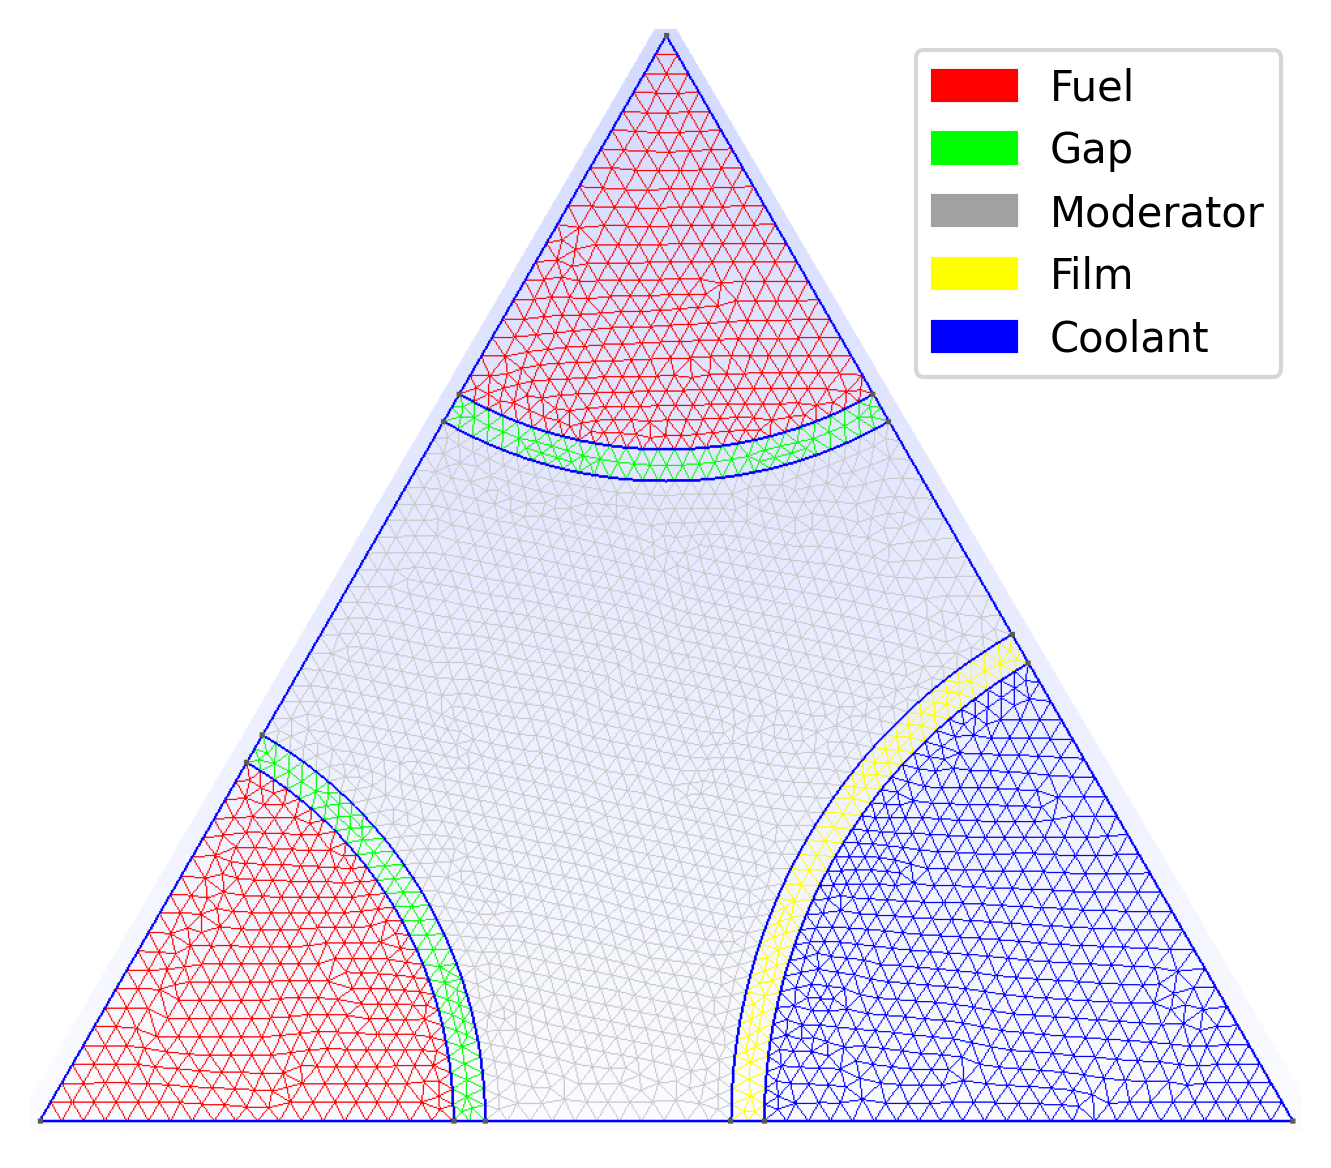
\includegraphics[width=0.40\textwidth]{figures-thermal/val-unit-mesh}
    }
    \subfloat[Material properties.]{
        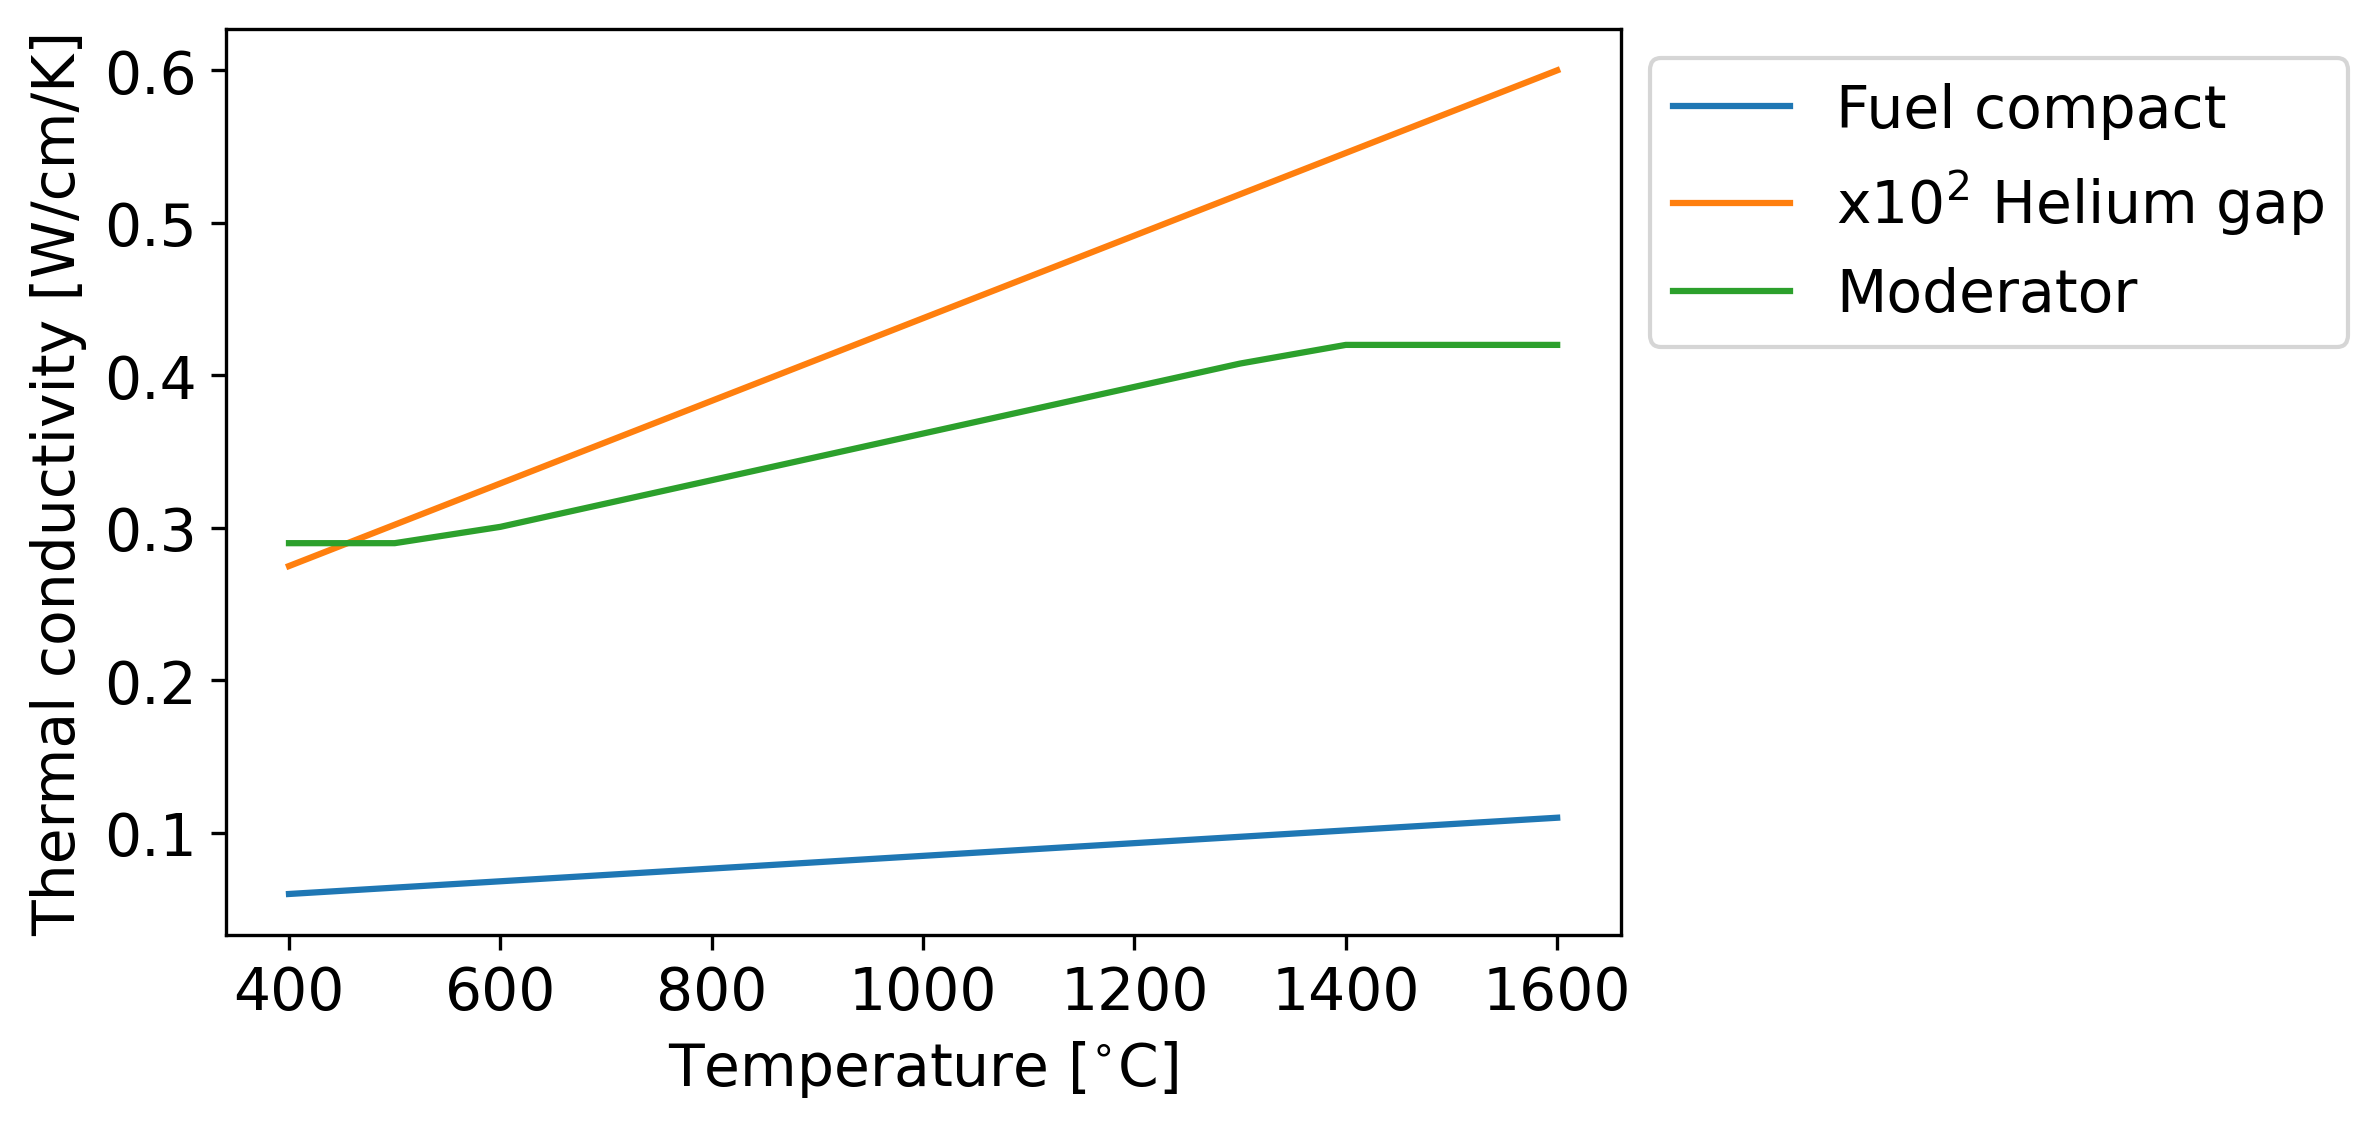
\includegraphics[width=0.50\textwidth]{figures-thermal/val-unit-matprop}
    }
	\hfill
	\label{fig:th-val-unit-model}
\end{figure}

Figure \ref{fig:th-val-unit-temps} shows the temperature profiles.
The axial temperatures increase from the top to the bottom of the reactor.
The moderator and coolant temperatures are parallel as the model assumes a film thermal conductivity independent of the temperature.
The fuel and moderator temperature difference decreases.
As the thermal conductivities of the different materials increase with temperature, the thermal resistance between the moderator and the fuel decreases.
Table \ref{fig:th-val-unit-results} summarizes the results.
Moltres/MOOSE coolant temperature is smaller by 4$^{\circ}$C.
The moderator temperature is larger by 9$^{\circ}$C.
The fuel temperature is larger by 22$^{\circ}$C.
The cause of this is the power profile simplification.
For a sinusoidal power profile the fuel-to-coolant temperature difference is small in the outlet, as we have seen in the previous section.
The opposite scenario is the uniform power profile, where the fuel-to-coolant temperature difference is larger.
In et al. used a chopped cosine power profile which we can think of it as the case in between a uniform and a sinusoidal power profile.
Overall, our model results showed good agreement with In et al. results.

\begin{figure}[htbp!]
  \centering
    \subfloat[Maximum fuel, moderator, and bulk coolant axial temperatures.]{
        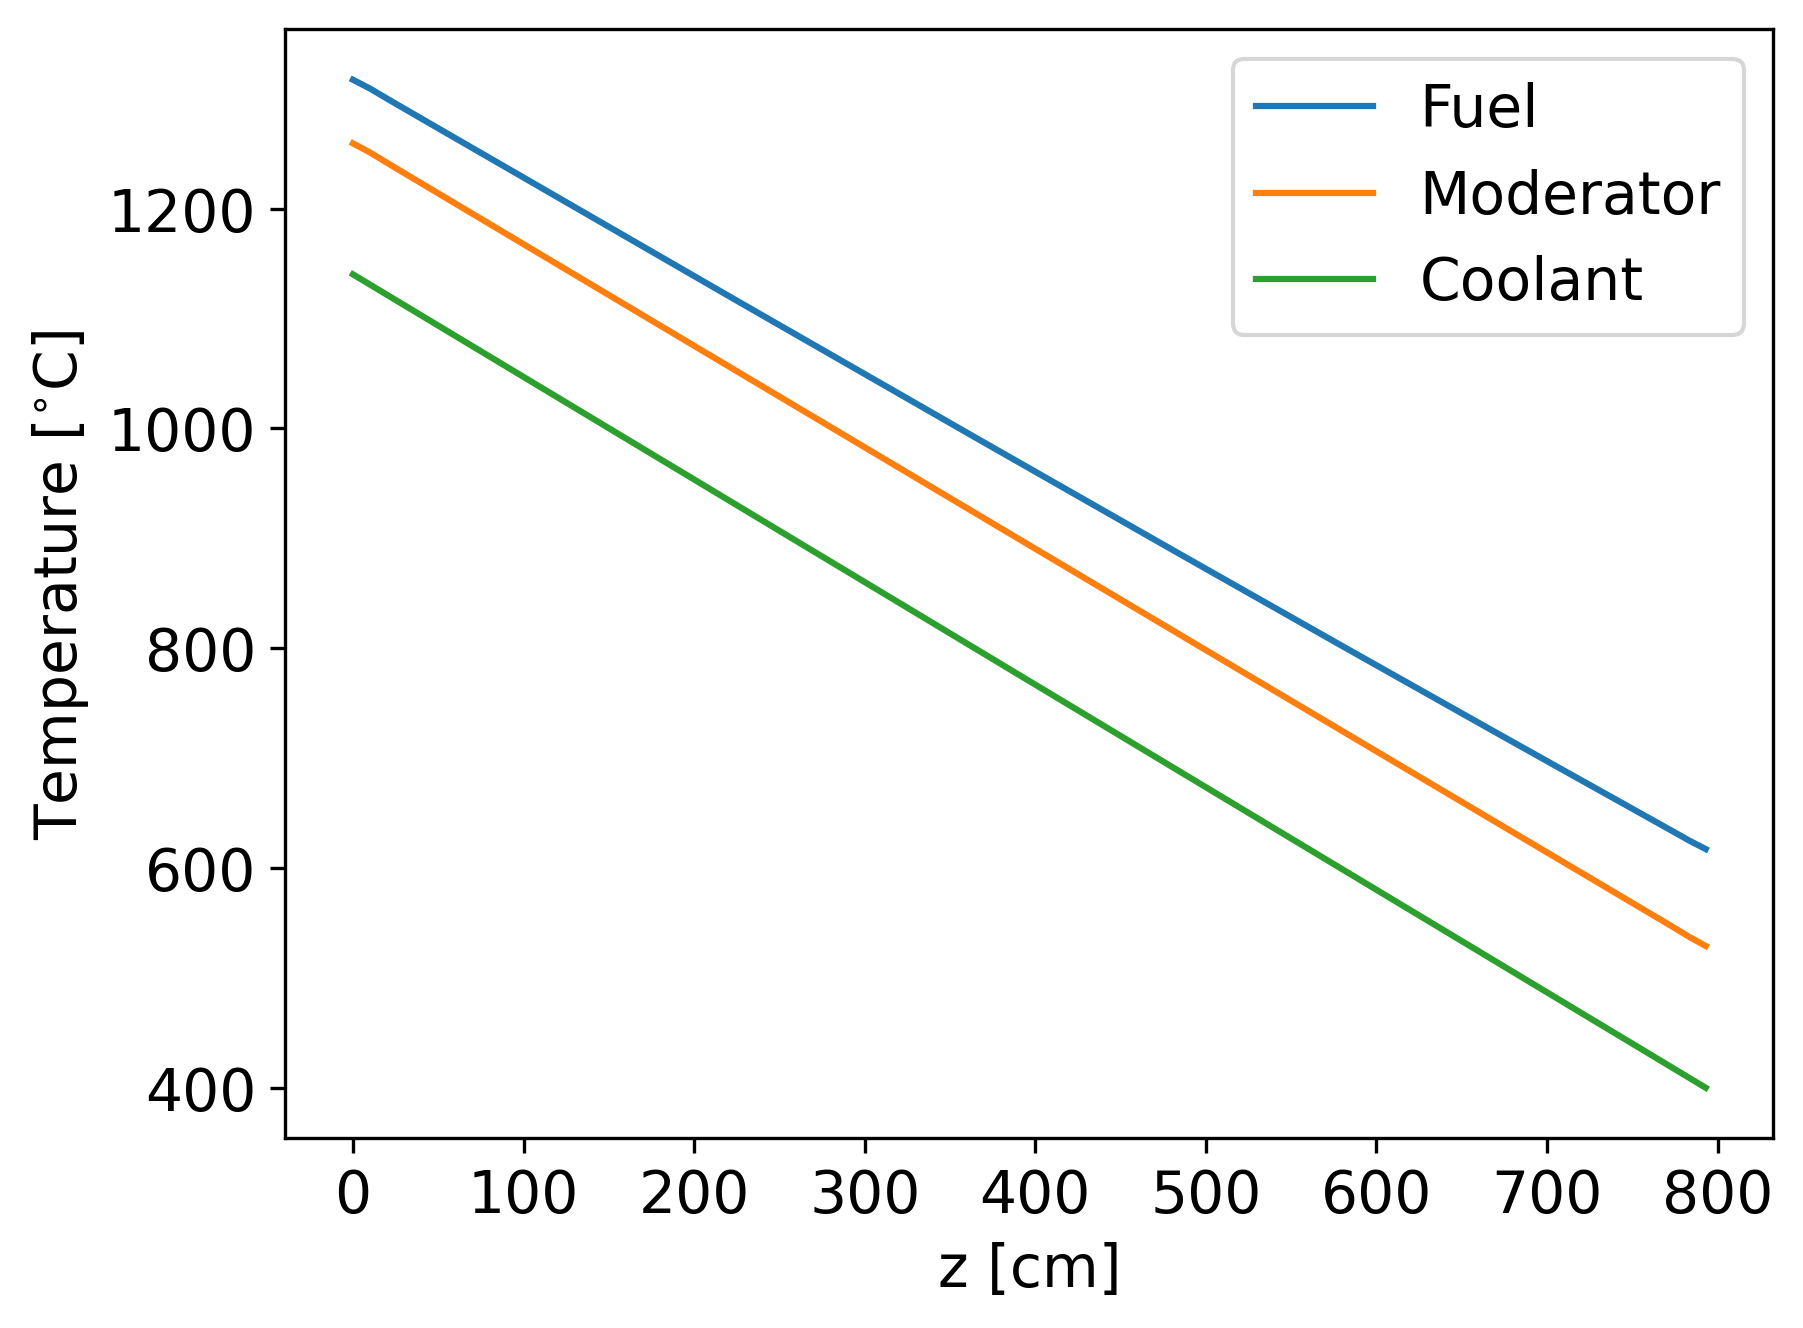
\includegraphics[width=0.45\textwidth]{figures-thermal/in-2006-5-axial}
    }
    \subfloat[Outlet plane temperature z=793 cm.]{
        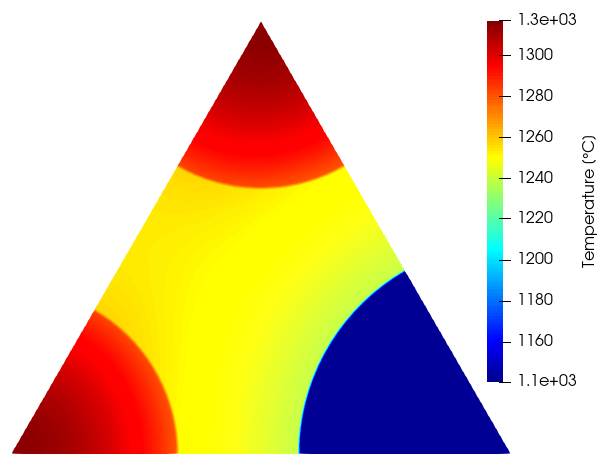
\includegraphics[width=0.45\textwidth]{figures-thermal/val-unit-outlet-plane}
    }
  \hfill
    \caption{Temperature profiles.}
  \label{fig:th-val-unit-temps}
\end{figure}

\begin{table}[htbp!]
\centering
      \caption{Maximum temperatures.}
      \label{tab:th-val-unit-results}
    \begin{tabular}{@{}l c c}
    \toprule
  Parameter   & In et al. 2006 \cite{in_three-dimensional_2006} & Moltres/MOOSE \\
    \midrule
  Maximum coolant temperature [$^{\circ}$C]   & 1144 & 1140 \\
  Maximum moderator temperature [$^{\circ}$C] & 1250 & 1259 \\
  Maximum fuel temperature [$^{\circ}$C]      & 1295 & 1317 \\
    \bottomrule
  \end{tabular}
\end{table}

\section{Fuel assembly}

This section aims to reproduce some of the analyses in Sato et al. 2010 \cite{sato_computational_2010}.
The study uses the GT-MHR as the reference reactor for the calculations.
The GT-MHR shares the geometry specifications with the MHTGR.
Table \ref{tab:element-characteristics} specifies the fuel element geometry.

Material properties from \cite{johnson_cfd_2009}.

The moderator is graphite H-451.
Fuel compact and moderator thermal conductivities displayed in \ref{tab:th-val-assem-mat}.
Helium thermal conductivity from \cite{nist_thermophysical_2020}.

Figure \ref{fig:th-val-assem-model} displays the model geometry and the model material properties that depend on the temperature.
Table \ref{tab:th-val-assem-massflow} shows the mass flow rate in each coolant channel.

\begin{table}[htbp!]
\centering
      \caption{Problem characteristics.}
      \label{tab:th-val-unit-char}
    % \begin{tabular}{@{}l c S[table-format=2.2] c c}
    \begin{tabular}{@{}l c c c c}
    \toprule
    \multicolumn{1}{c}{Parameter} & \multicolumn{1}{c}{Symbol} & \multicolumn{1}{c@{}}{Value} & \multicolumn{1}{c@{}}{Units} & \multicolumn{1}{c}{Reference} \\
    \midrule
  Inlet coolant temperature & T$_{in}$  & 490   & $^{\circ}$C   & \cite{sato_computational_2010} \\
  Helium inlet pressure     & P         & 70    & bar           & \cite{sato_computational_2010} \\
  Helium density            & $\rho$    & 4.37 $\times 10^{-6}$ & kg/cm$^3$ & \cite{nist_thermophysical_2020} \\
  Helium heat capacity      & c$_p$     & 5188  & J/kg/K        & \cite{nist_thermophysical_2020} \\
  Average power density     & q$_{ave}$ & 27.88 & W/cm$^3$      & \cite{sato_computational_2010} \\
    \midrule
  \multicolumn{1}{c}{Calculated parameters} &  &  &  & \\  
    \midrule
  Coolant film radius       & R$_i$ & 0.804    & cm     & -  \\
  Film thermal conductivity & k$_i$ & 2.09 $\times 10^{-3}$ & W/cm/K & -  \\
  \bottomrule
  \end{tabular}
\end{table}

\begin{table}[htbp!]
\centering
  \caption{Thermal conductivity coefficients.}
  \label{tab:th-val-assem-mat} 
  \begin{tabular}{c|ccc|c}
\toprule
                          & \multicolumn{3}{c|}{Moderator}         & Fuel compact \\ \hline
Temperature range {[}K{]} & 255.6-816 & 816-1644.4 & 1644.4-1922.2 & 255.6-2200   \\
\midrule
A1                        & 28.6      & 1.24E+2    & 41.5          & 3.94         \\
A2                        & -         & -3.32E-1   & -             & 3.59E-3      \\
A3                        & -         & 4.09E-4    & -             & -1.98E-9     \\
A4                        & -         & -2.11E-7   & -             & 3.19E-12     \\
A5                        & -         & 4.02E-11   & -             & -9.77E-16    \\
\bottomrule
  \end{tabular}
\end{table}

\begin{figure}[htbp!]
  \centering
    \subfloat[Model geometry.]{
        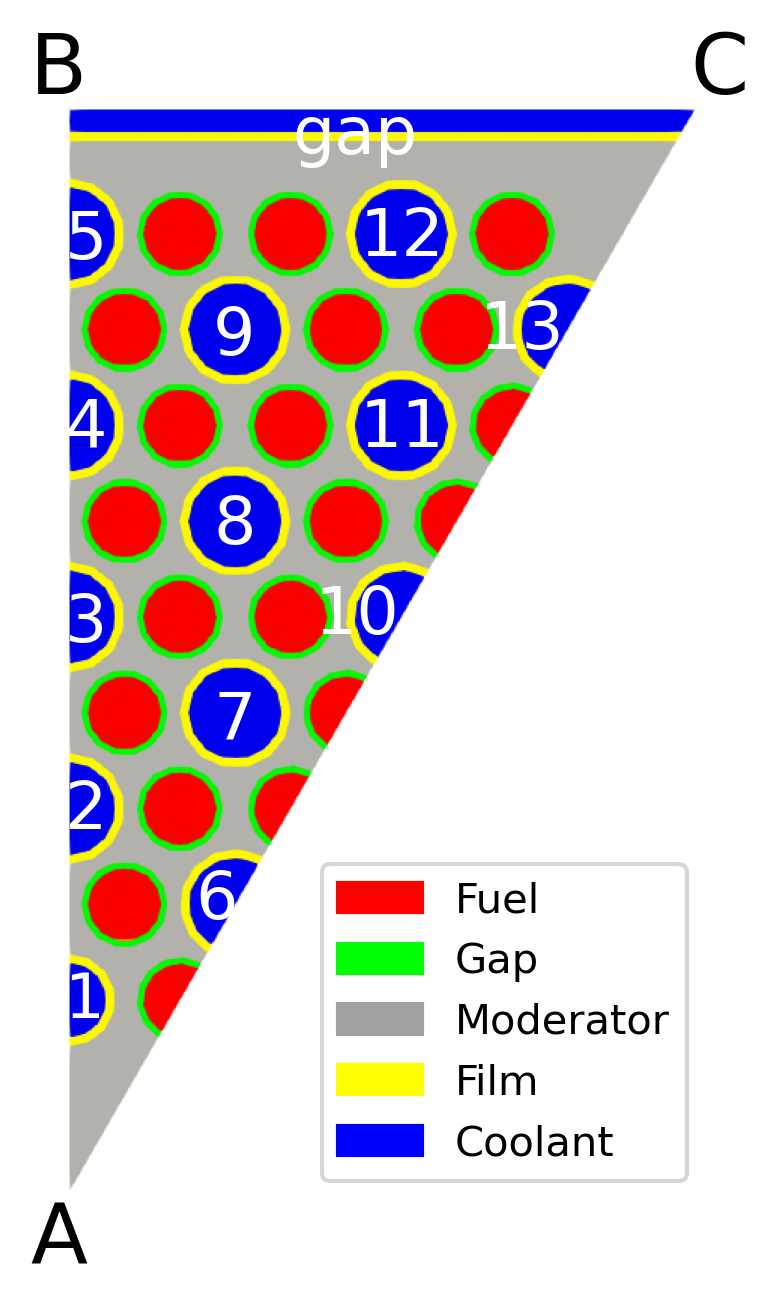
\includegraphics[width=0.45\textwidth]{figures-thermal/val-assem-mesh}
    }
    \subfloat[Material properties.]{
        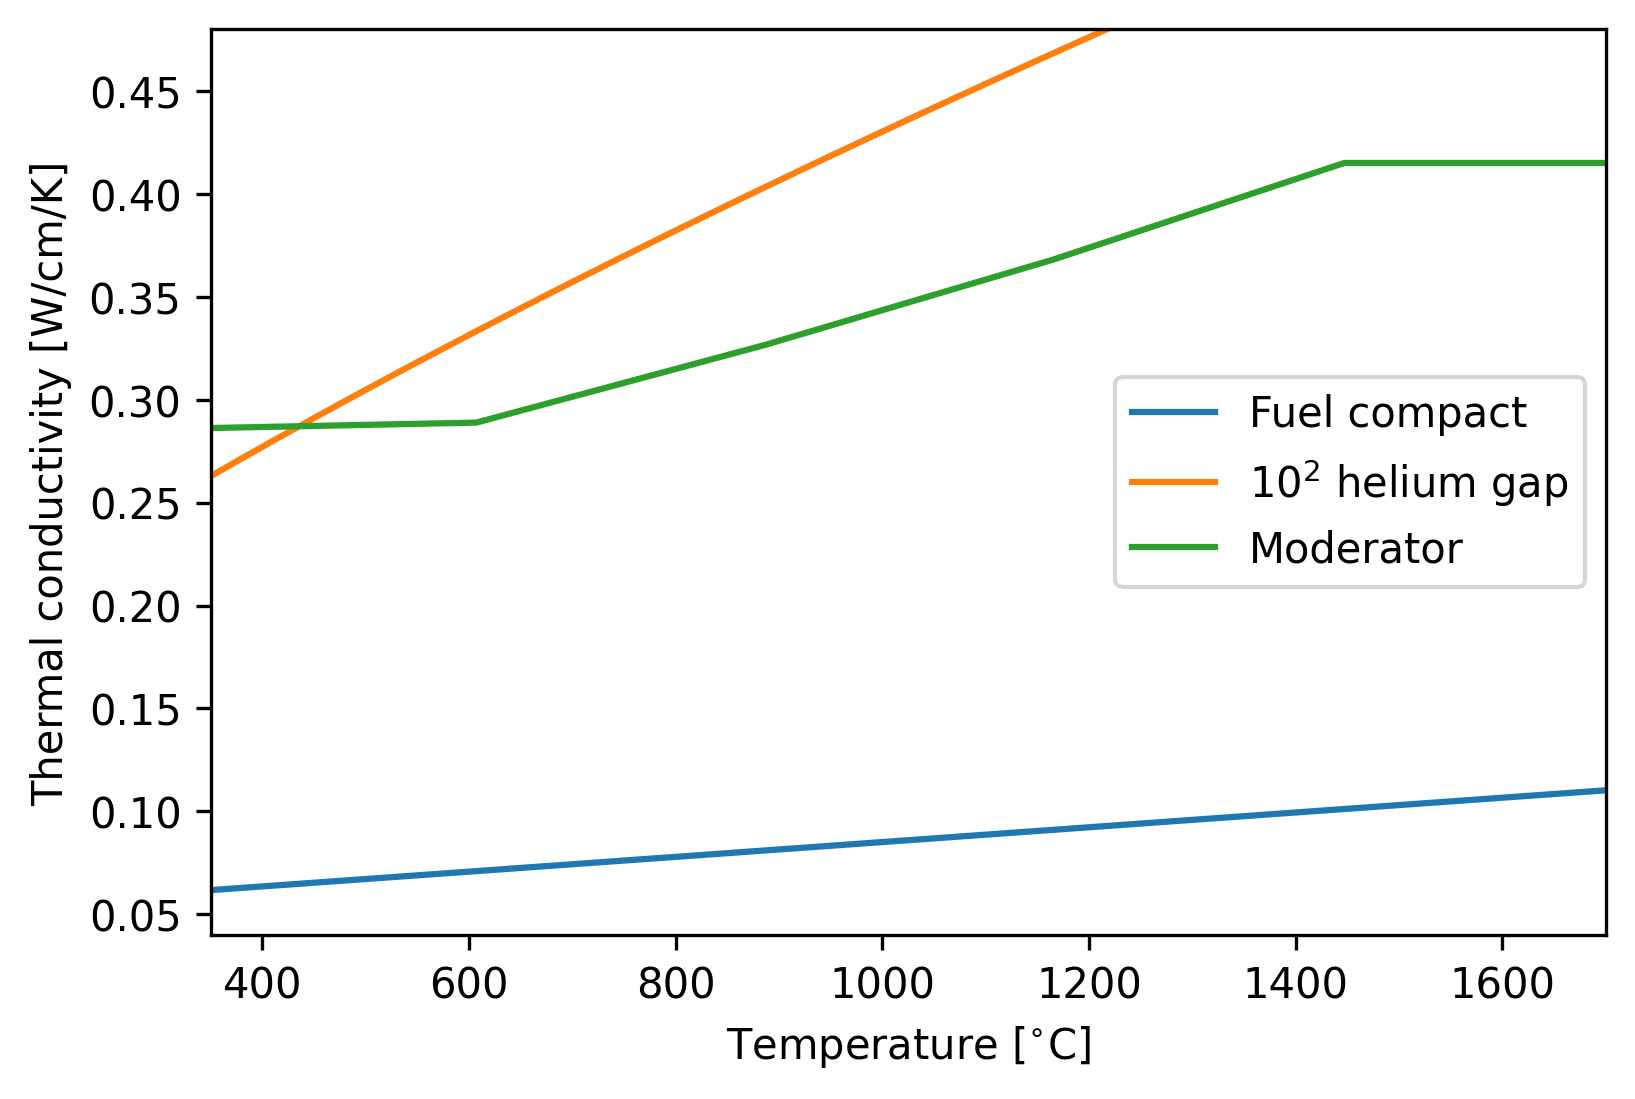
\includegraphics[width=0.45\textwidth]{figures-thermal/val-assem-matprop}
    }
  \hfill
  \label{fig:th-val-assem-model}
\end{figure}

\begin{table}[htbp!]
\centering
  \caption{Mass flow rate [g/s]. Values form \cite{sato_computational_2010}.}
  \label{tab:th-val-assem-massflow}
  \begin{tabular}{lllllllllllllll}
\toprule
Channel & 1 & 2 & 3 & 4 & 5 & 6 & 7 & 8 & 9 & 10 & 11 & 12 & 13 & Gap \\
\midrule
No gap  & 6.18 & 11.34 & 11.37 & 11.38 & 11.43 & 11.33 & 22.70 & 22.73 & 22.73 & 11.38 & 22.77 & 22.91 & 11.44 & -     \\
3mm gap & 5.88 & 10.80 & 10.85 & 10.91 & 11.08 & 10.80 & 21.58 & 21.67 & 21.83 & 10.88 & 21.81 & 22.20 & 11.10 & 16.56 \\
\bottomrule
\end{tabular}
\end{table}

Table \ref{tab:th-val-assem-results}
Figure \ref{fig:th-val-assem-temps}

\begin{table}[htbp!]
  \centering
  \caption{Maximum temperatures.}
  \label{tab:th-val-assem-results}
\begin{tabular}{l|ll|ll}
\toprule
                                   & \multicolumn{2}{l|}{No gap} & \multicolumn{2}{l}{3mm gap} \\ \midrule
                                   & Sato et al. & Moltres/MOOSE & Sato et al. & Moltres/MOOSE \\ \midrule
Maximum fuel temperature           & 1090    & 1094              & 1115     & 1114             \\
Maximum outlet coolant temperature & 985     & 983               & 1007     & 1005               
\bottomrule
\end{tabular}
\end{table}

\begin{figure}[htbp!]
  \centering
    \subfloat[Line A-B.]{
        \includegraphics[width=0.45\textwidth]{figures-thermal/val-assem-lineAB}
    }
    \subfloat[Line A-C.]{
        \includegraphics[width=0.45\textwidth]{figures-thermal/val-assem-lineAC}
    }
  \hfill
  \caption{Outlet plane temperature along the line A-B and line A-C.}
  \label{fig:th-val-assem-temps}
\end{figure}

% \begin{figure}[htbp!]
%   \centering
%     \subfloat[No gap.]{
%         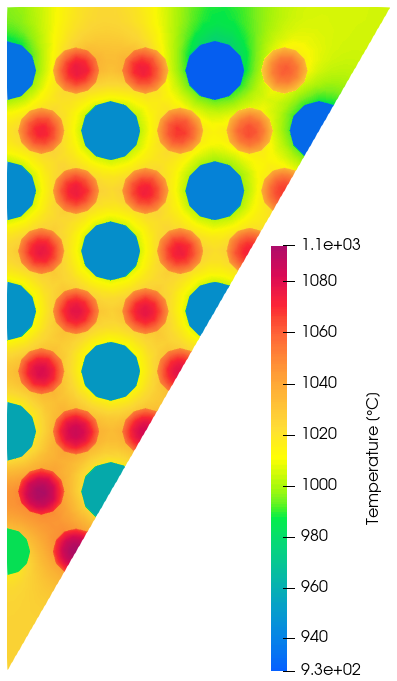
\includegraphics[width=0.45\textwidth]{figures-thermal/val-assem-input}
%     }
%     \subfloat[3mm gap.]{
%         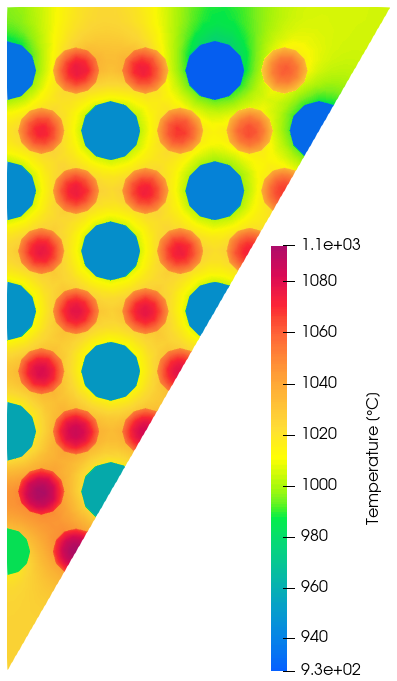
\includegraphics[width=0.45\textwidth]{figures-thermal/val-assem-input}
%     }
%   \hfill
%   \caption{Outlet plane temperature profile.}
%   \label{fig:th-val-assem-temps}
% \end{figure}


\subsection{Flow distribution analysis}

Talk about the necessity for this capability.
Also mention the different exercises from the benchmark.

Compares mass flow and max coolant and fuel temperatures: w/ no gap (it would be better with the gap, but the previous analysis is still wrong sooooo)
- sato et al
- flat (same velocity across all the channels)
- incompressible
- acceleration term

This simplified algorithms allow for solving the mass flow rate distribution in the core for steady-state cases, and for transient cases as an approximation.
However, in coupled analyses, the flow distribution depends on the temperature and will change along time.
This creates the necessity for developing tools integrated into Moltres.
Currently, MOOSE has a module for modeling the incompressible Navier-Stokes equations.
Integrating that module into the solver could improve the accuracy.
This task will be part of the future work.

\section{Full core}

This section will extend the methodology to a full-core problem and it will intend to solve Exercise 2 of Phase I of the OECD/NEA MHTGR-350 Benchmark.

\section{Neutronics and Thermal-fluids Coupling}

3 options:
- Heterogeneous model
- Homogenized media and sub-channel unit cell model: how does it solve advection ?
- Porous media model
